\documentclass{beamer-control}
\usepackage{beamer-control-singlefile}
\INCLUDEONLY{The Bode Plot}
\begin{document}
\CONCEPT{The Bode Plot}

\begin{SUMMARY}
\begin{itemize}
\item Sketching and Interpreting Bode Plots
\item Poles and Zeros in the Right Half-Plane
\item Time Delays
\item System Insights from the Bode Plot
\item Determining Transfer Functions Experimentally
\end{itemize}
\vfill References:
\begin{itemize}
\item \astrom{§9.6}
\end{itemize}
\end{SUMMARY}


\begin{frame}
\frametitle{Introduction}
The \alert{frequency response} of a system is computed from its transfer function with $s=\ii\ww$, which corresponds to an input of:
\begin{align}
u(t) = \Exp{\ii\ww t} = \cos \ww t + \ii \sin \ww t
\end{align}
We have seen the resulting output is
\begin{align}
y(t) = G(\ii\ww)\Exp{\ii\ww t} = M\cos(\ww t+\theta) + \ii M \sin(\ww t + \theta)
\end{align}
which use the gain $M$ and phase $\theta$ of $G$ defined as:
\begin{align}
M &= \abs (G(\ii\ww)) & \theta &= \arg( G(\ii\ww)) = \arctan \frac{\Imag G(\ii\ww)}{\Real G(\ii\ww)}
\end{align}
We can visualise $M$ and $\theta$ versus frequency --- the Bode Plot
\end{frame}

\begin{frame}{Calculating the FR analytically}
  \begin{itemize}
    \item  Start with transfer function $F(s)$\\ (mathematically $F(s)\colon\mathbb{C}\to\mathbb{C}$)
    \item  Substitute $s=\jj\ww$ \qquad --- n.b.\ real frequencies only
    \item  (If by hand, separate $F(\ww)$ into real and complex components)
    \item  Create a vector of frequencies $\ww\in\{\omega_0,\omega_1,\omega_2,\dots\}$
    \item  Calculate vector of responses $\bigl\{F(\omega_0),F(\omega_1),F(\omega_2),\dots\bigr\}$
  \end{itemize}
\end{frame}

\begin{frame}{Example}
  \begin{align*}
  G &= \frac{10}{s+5}
    = \frac{10}{5+\jj\ww}
     = \frac{10(5-\jj\ww)}{(5+\jj\ww)(5-\jj\ww)}
     = \frac{50}{25+\ww^2} + \jj\frac{-10\ww}{25+\ww^2}
  \end{align*}
  \bigskip
  \begin{align*}
  \Real(G(\ww)) & = \frac{50}{25+\ww^2} &
  \lvert G(\ww)\rvert & = \frac{\sqrt{2500+100\ww^2}}{25+\omega^2} \\
  \Imag(G(\ww)) & = \frac{-10\ww}{25+\ww^2} &
  \measuredangle G(\ww) & = \arctan(-10\ww/50)
  \end{align*}
\end{frame}

\begin{frame}
\frametitle{Example Bode Plot}
\centering
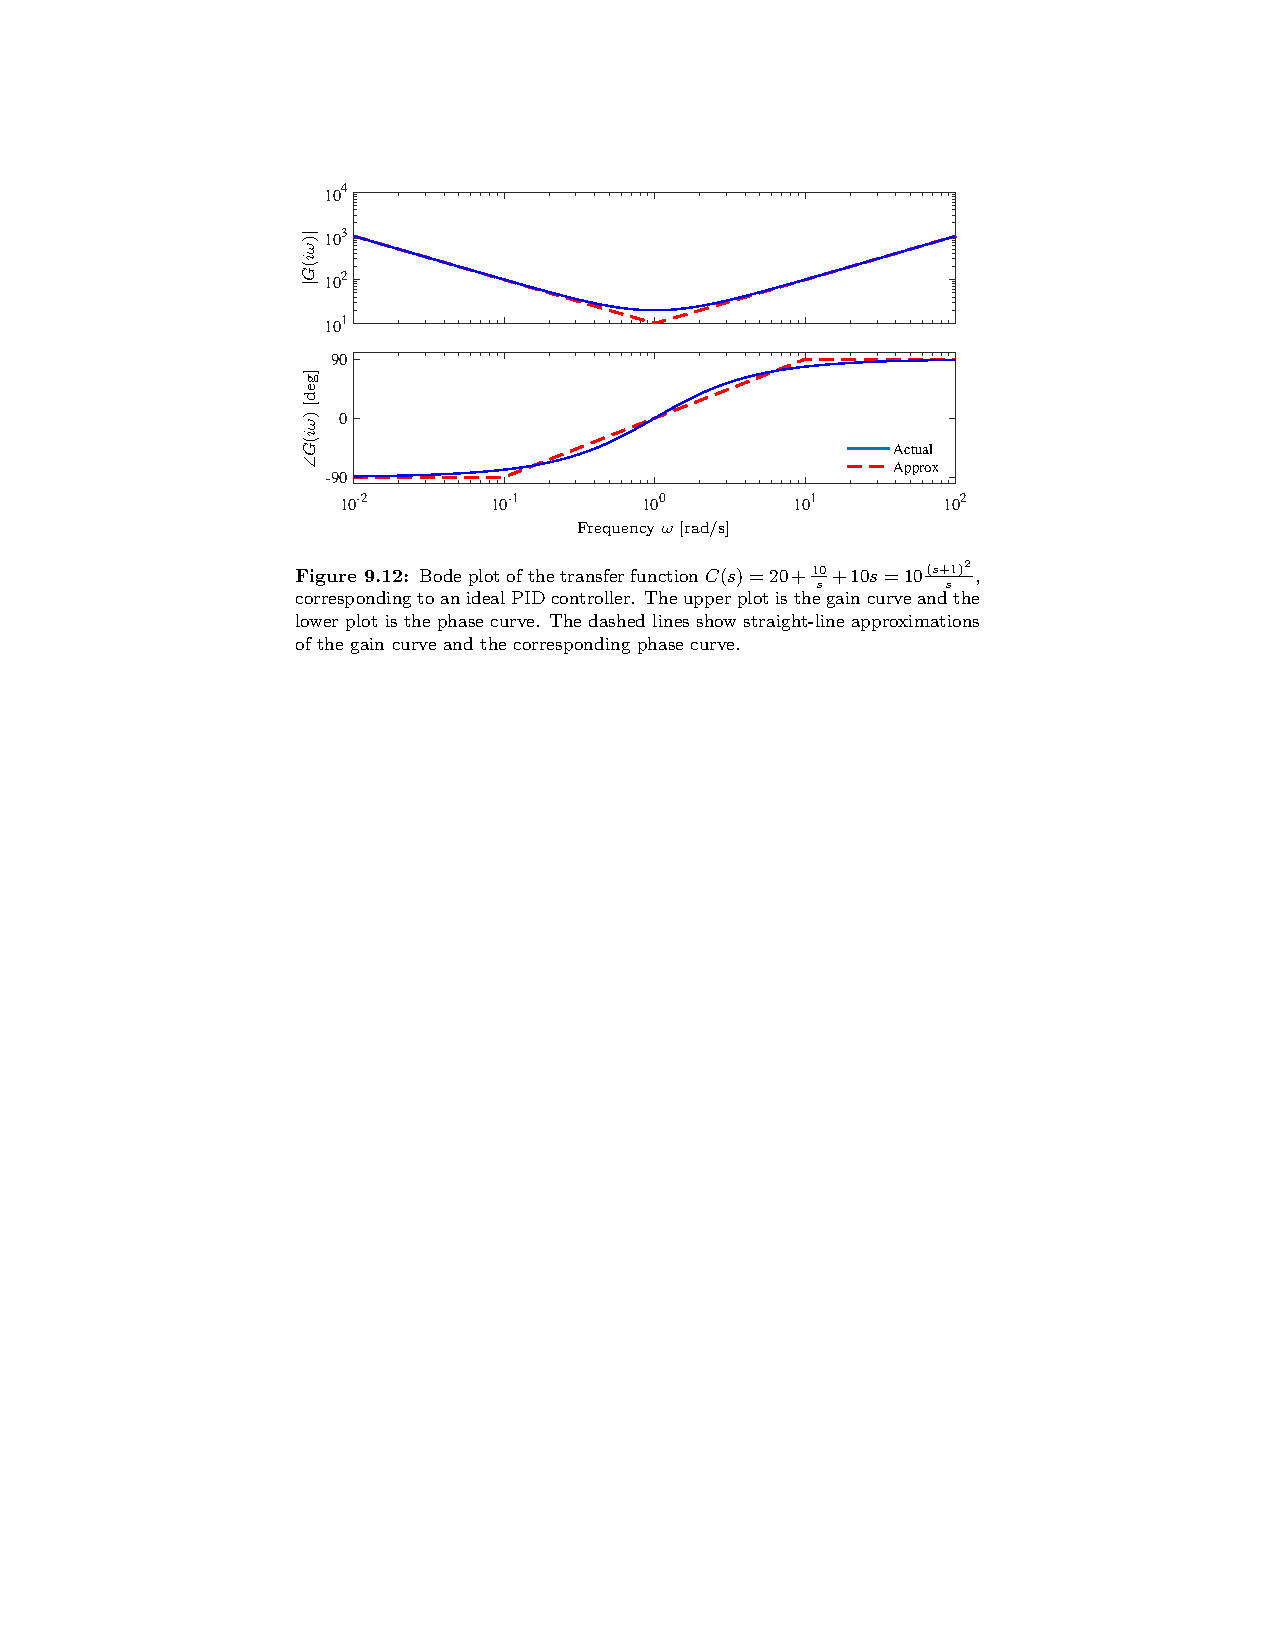
\includegraphics[width=0.8\linewidth]{figure9.12}

\end{frame}

\SUBCONCEPT{Sketching and Interpreting Bode Plots}

\begin{frame}{Canonical Bode Plots --- integrator and differentiator}
\centering
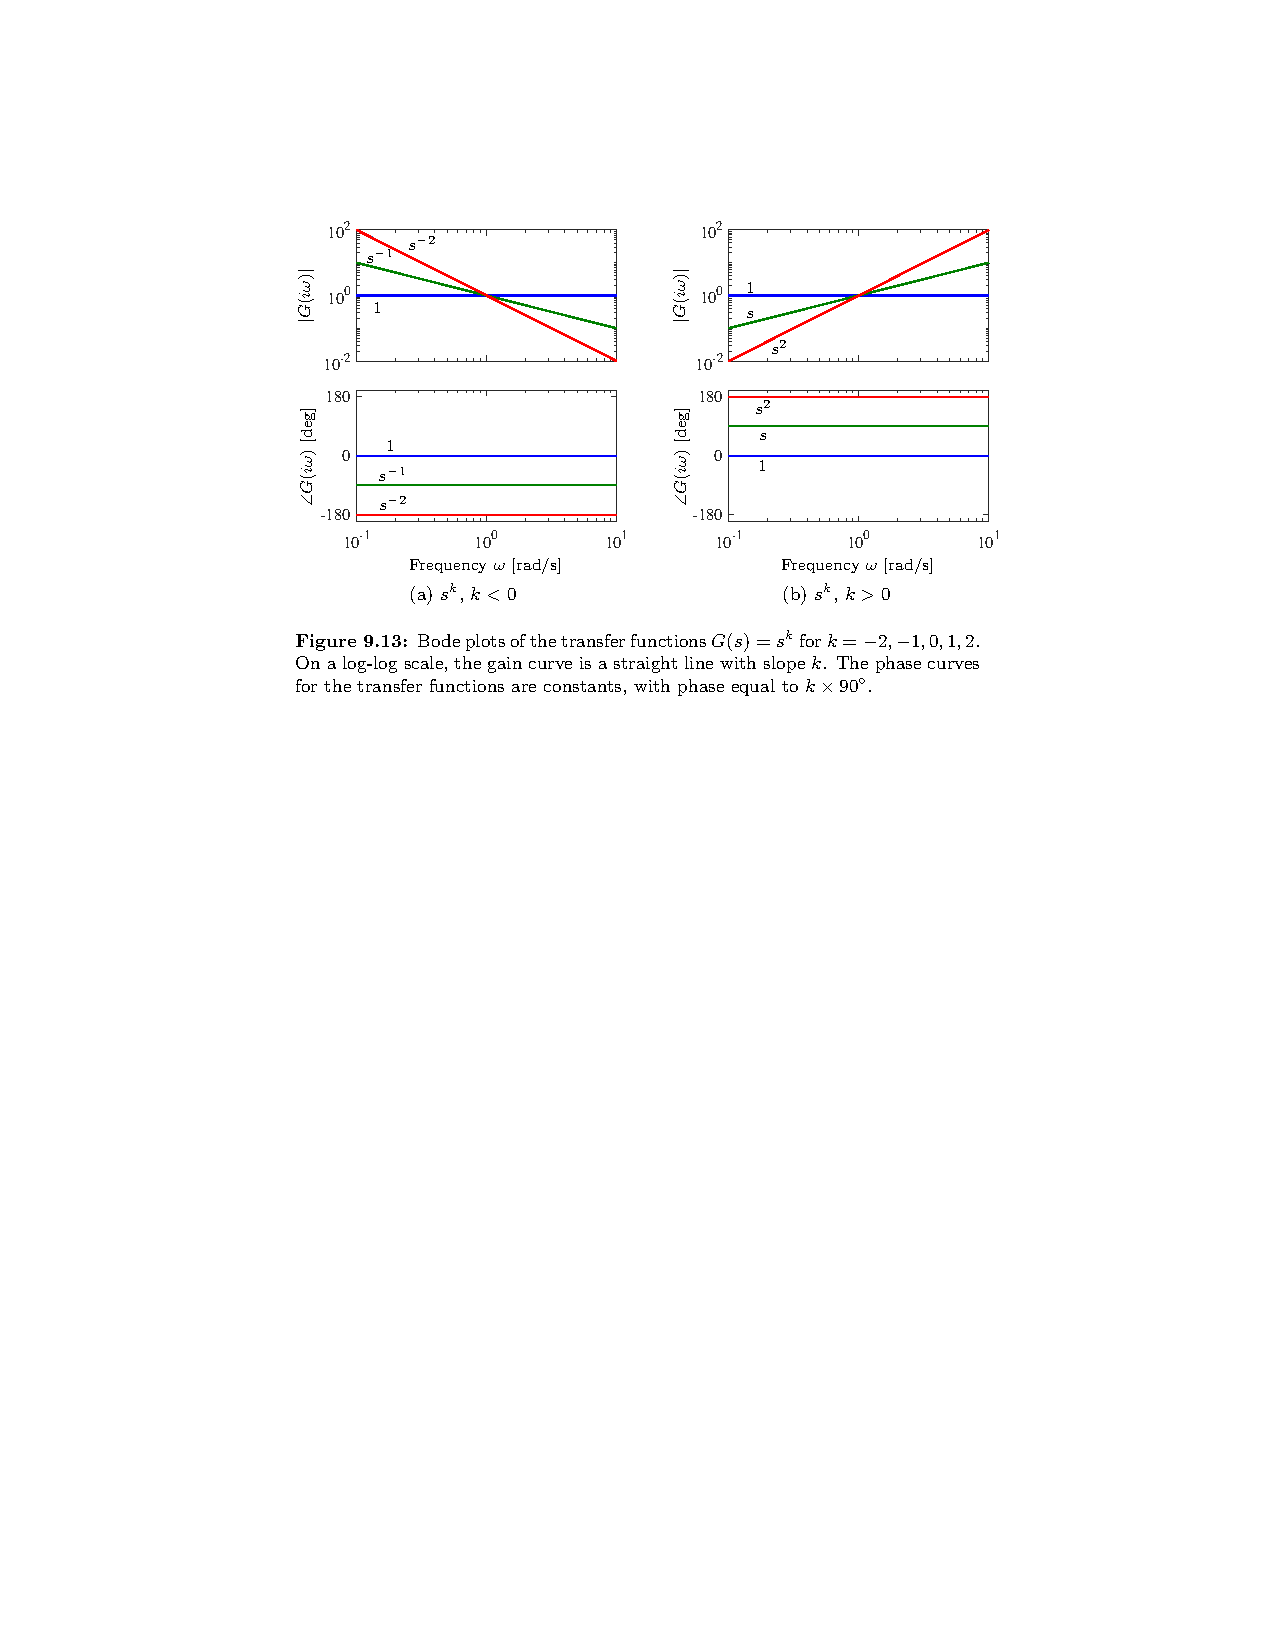
\includegraphics[height=0.8\textheight]{figure9.13}

\end{frame}

\begin{frame}{Canonical Bode Plots --- first order and second order}
\centering
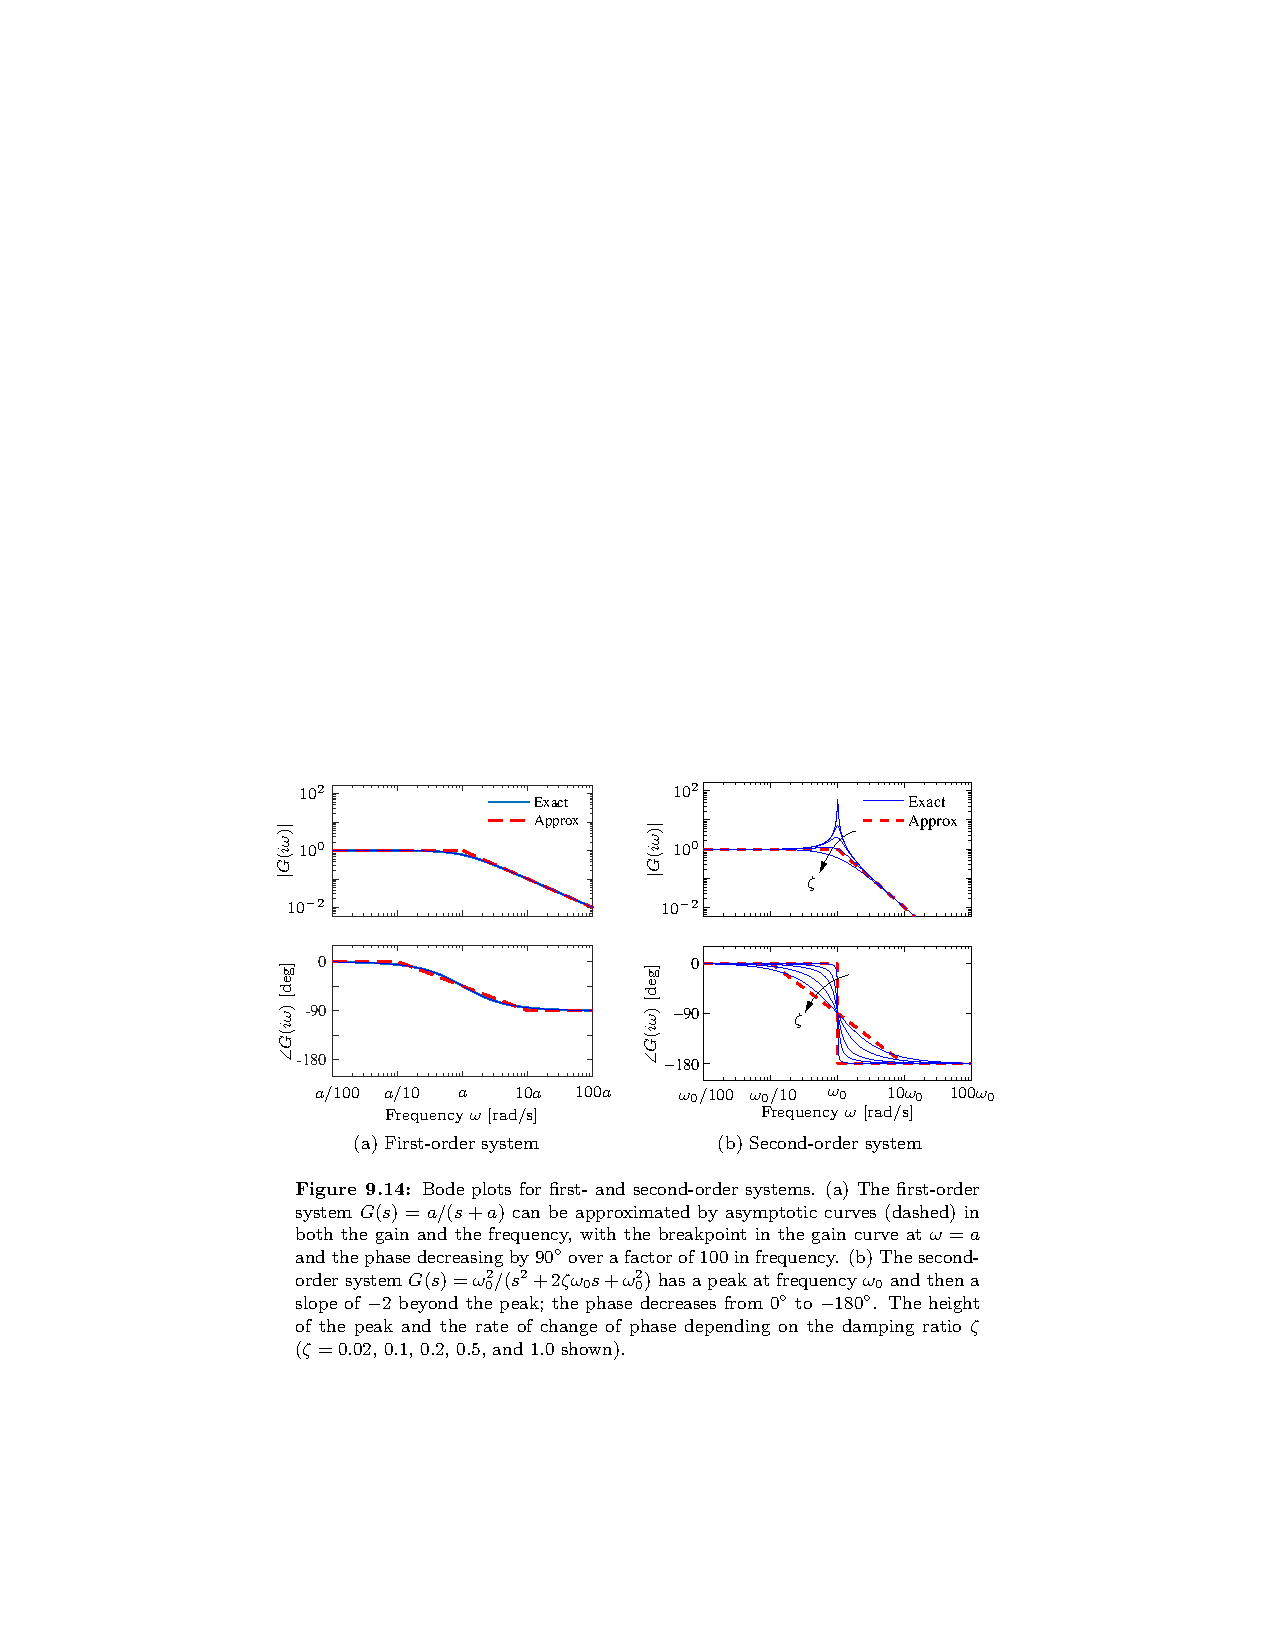
\includegraphics[height=0.8\textheight]{figure9.14}

\end{frame}

\begin{frame}{Example Bode Plot --- 1 zero, 3 pole system}
\centering
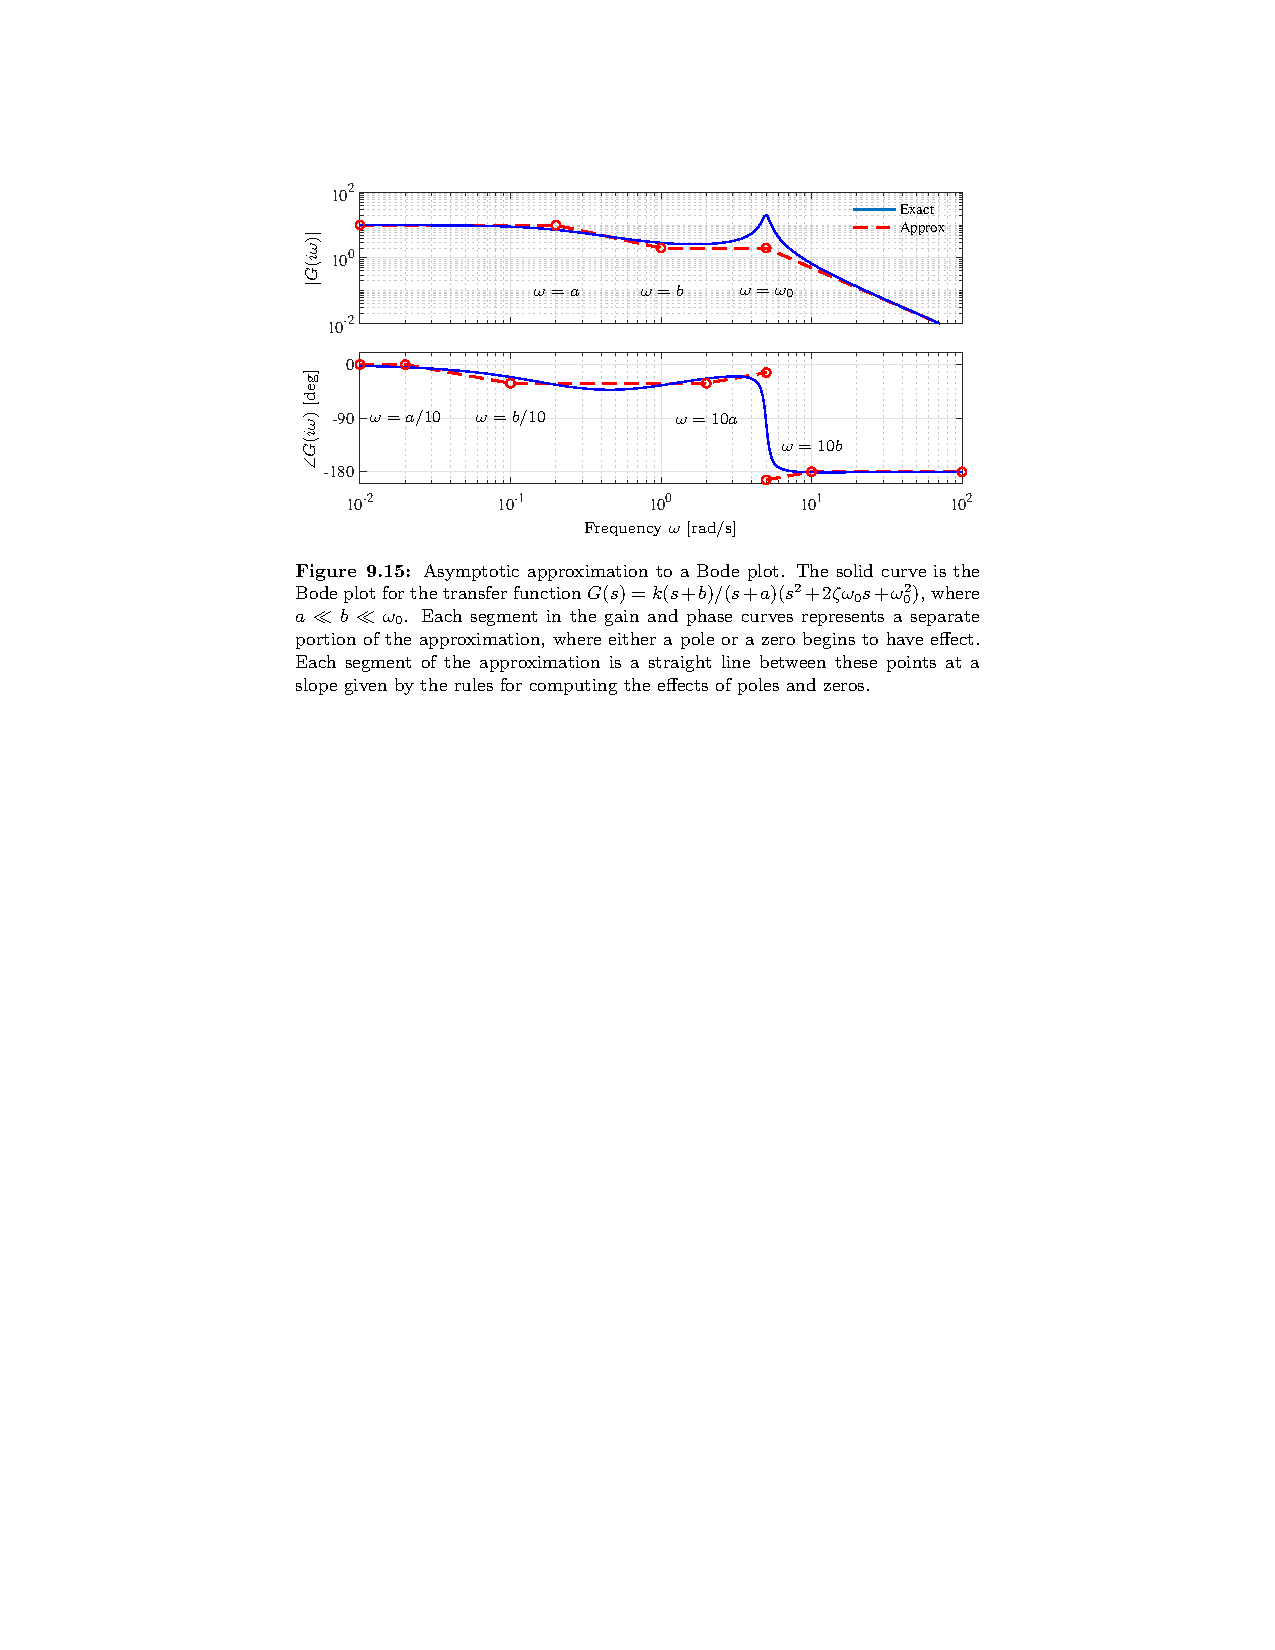
\includegraphics[height=0.8\textheight]{figure9.15}

\end{frame}




\begin{frame}
\begin{columns}
\column{0.4\linewidth}
\[
  GH = \frac{100(s+1)}{(s+10)(s+100)}
\]
\bigskip
\emph{In Matlab:}

\includematlab{topic5/bode1.m}{bode2}

\bigskip
{\tiny Actually the plot on the right is done a little more carefully.\par}

\column{0.6\linewidth}
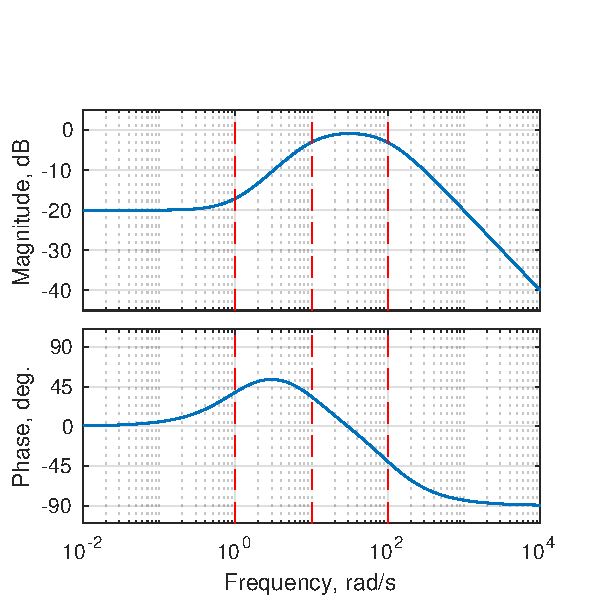
\includegraphics[width=\linewidth,clip,trim=0 0 0 30]{bode1.pdf}
\end{columns}
\end{frame}


\begin{frame}{Summary of rules}
  Magnitude:
  \begin{itemize}
    \item  Starts at magnitude of DC gain
    \item  Start with `flat' slope of \SI{0}{dB/dec}
    \item  One pole: add $-\SI{20}{dB/dec}$ slope
    \item  One zero: add $+\SI{20}{dB/dec}$ slope
  \end{itemize}
  Phase:
  \begin{itemize}
    \item  Start at \ang{0}
    \item  One pole: transition through $-\ang{90}$ (over one decade)
    \item  One zero: transition through $+\ang{90}$ (over one decade)
  \end{itemize}
  Important point:
  \begin{itemize}
    \item  Integrator is a pole at $s=0$
    \item  Differentiator is a zero at $s=0$
    \item  Same rules apply
  \end{itemize}
\end{frame}


\begin{frame}{More on phase limits}{For stable plants with +ve DC gain}
\begin{columns}[t]
\small
\column{0.5\linewidth}
Low frequency phase limit:
\[
\theta_0 = -\ang{90}\times(N_I-N_D)
\]
where
\begin{itemize}
\item $N_I =$ number of integrators
\item $N_D =$ number of differentiators
\end{itemize}

\column{0.5\linewidth}
High frequency phase limit:
\[
\theta_\infty = -\ang{90}\times(N_P-N_Z)
\]
where
\begin{itemize}
\item $N_P =$ number of poles\\ (incl.\ integrators)
\item $N_Z =$ number of zeros\\ (incl.\ differentiators)
\end{itemize}
$n_{pe} = (N_P-N_Z)$ is used often and termed the `poles excess'


\end{columns}
\end{frame}


\SUBCONCEPT{Poles and Zeros in the Right Half-Plane}

\begin{frame}
\frametitle{Non-minimum phase zeros}
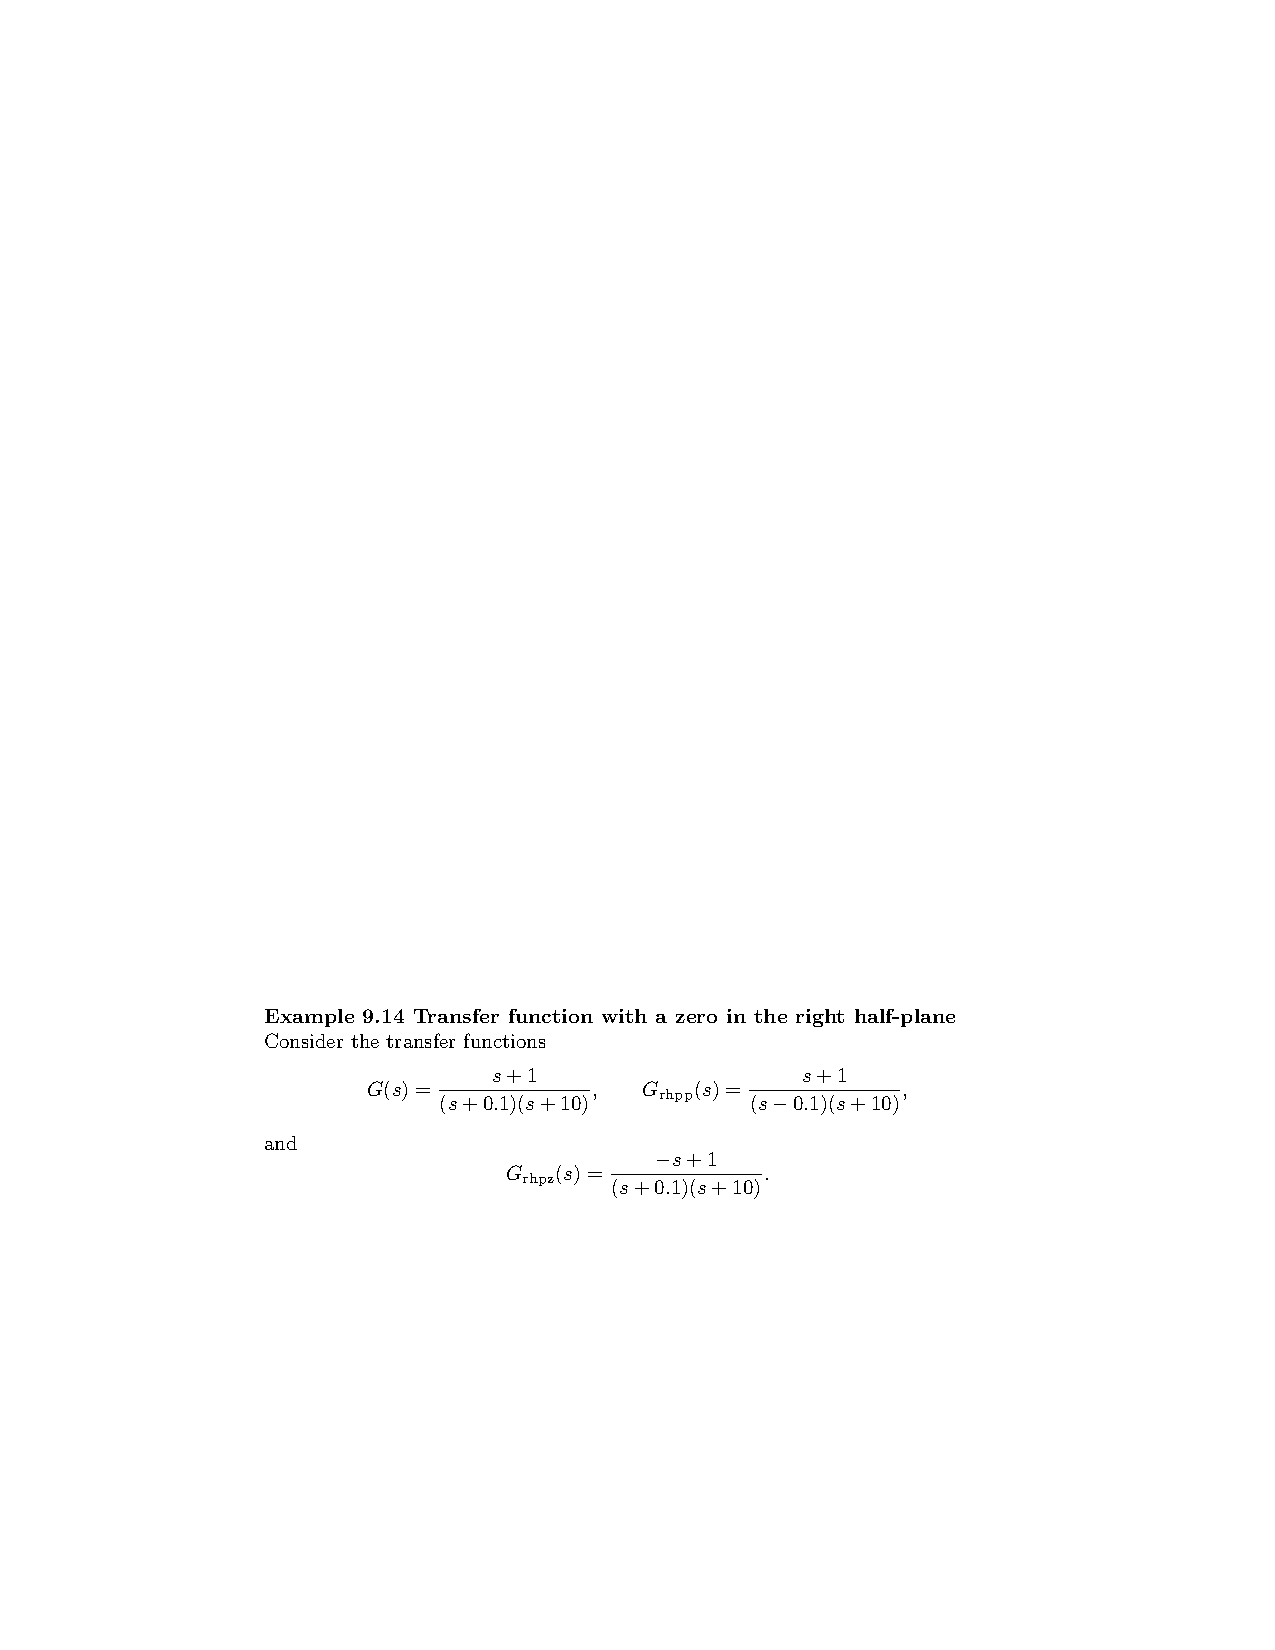
\includegraphics[width=0.8\linewidth]{example9.14}

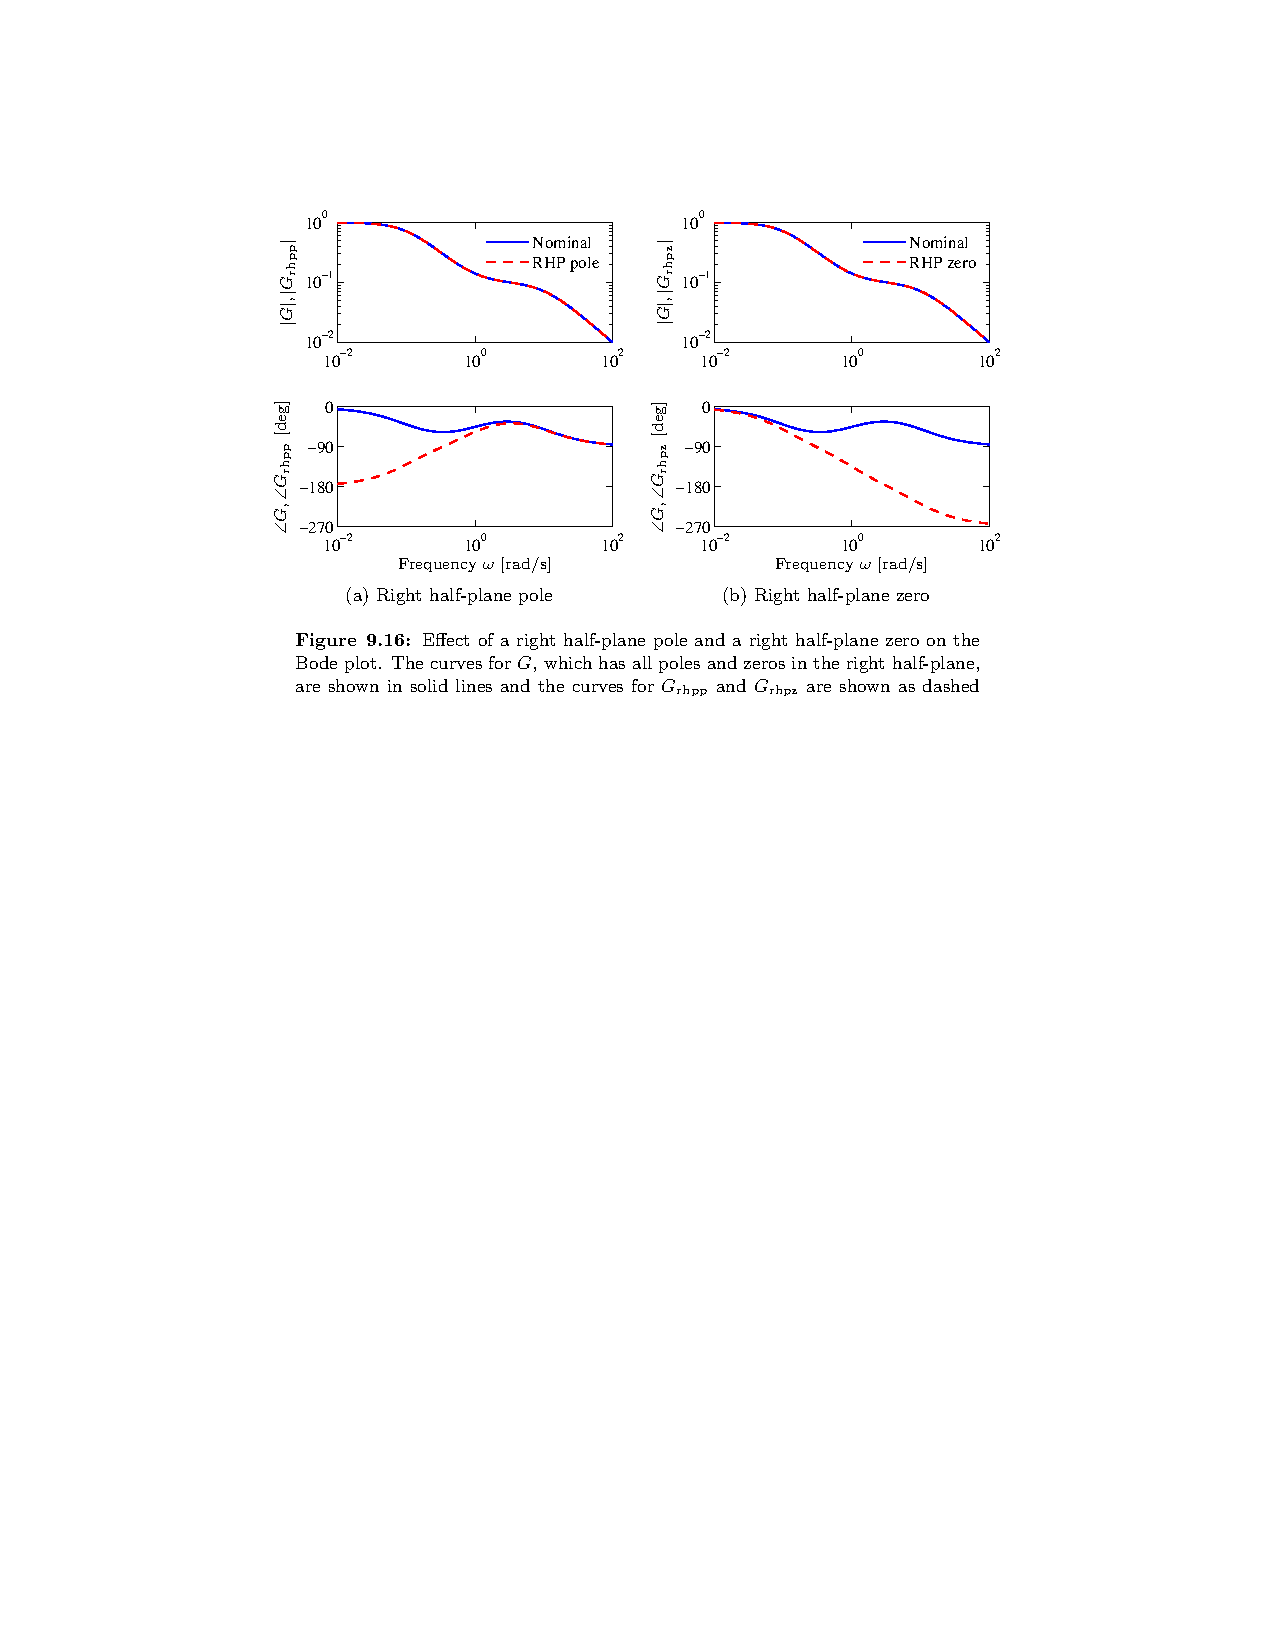
\includegraphics[width=0.8\linewidth]{figure9.16}

\end{frame}

\SUBCONCEPT{Time delays}

\begin{frame}
  \begin{itemize}
    \item  Time delays can cause stability problems
    \item  `Time delay' can mean:
    \begin{itemize}
      \item  Delays in reading data from a sensor
      \item  Delays in the control system
      \item  Delays in sending commands to the actuator
    \end{itemize}
    \item Can analyse problems from time delays but often can't overcome them with control
  \end{itemize}
\end{frame}

\begin{frame}{Pure delay}
\begin{columns}
\column{0.5\linewidth}
  \[
    G_{\mathrm{delay}} = \Exp{-s\tau}
  \]
\begin{itemize}
  \item No effect on magnitude
  \item $\theta_{\mathrm{delay}}=-\ww \tau$
  \item Reduces stability margins, leads to instability
\end{itemize}

\column{0.5\linewidth}
    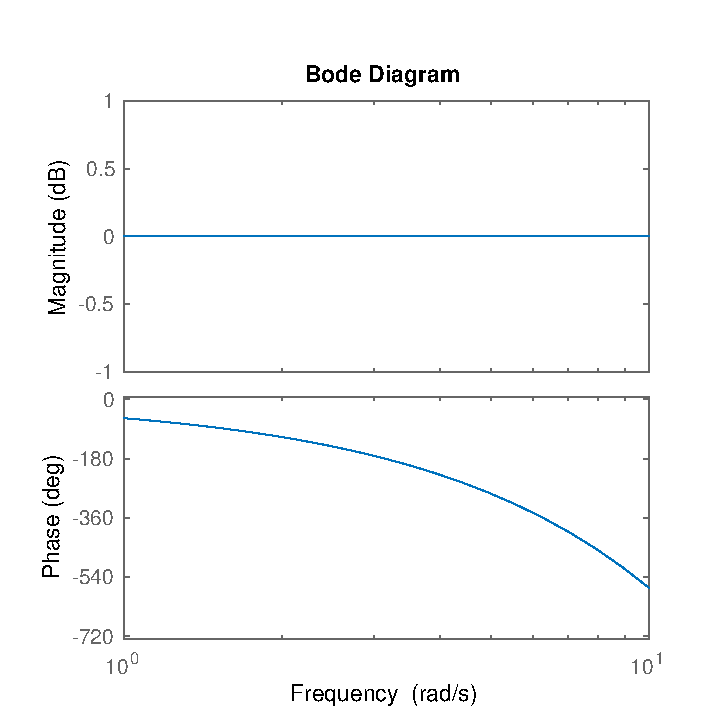
\includegraphics[width=\linewidth]{puretimedelaybode}
\end{columns}
\end{frame}

\begin{frame}
\frametitle{Padé approximation}
The exponential delay term $\exp(-s\tau)$ is not a rational function,
so we approximate it using the \alert{Padé approximation}.

This begins with the Maclaurin series of the delay, but we can't use this directly because truncating the series doesn't give us a well-behaved transfer function:
\begin{align}
\Exp{-s \tau} &= 1 - \tau s + \frac{1}{2!}(\tau s)^2 - \dots + \frac{(-1)^n}{n!}(\tau s)^n + \dots 
\end{align}

The Padé approximation of order $n$ is a ratio of polynomials that matches the series up to the same order:
\begin{align}\label{eq:pade}
\Exp{-s \tau} &\approx \mathrm{PD}(\tau,n) = \frac{ \sum_{k=0}^n (-1)^k c_k (\tau s)^k  }
                            { \sum_{k=0}^n        c_k (\tau s)^k  } \,, &
          c_k &= \frac{ (2n-k)!n! }{ (2n)!k!(n-k)! }
\end{align}

\end{frame}

\begin{frame}
\frametitle{Just in case that equation is not self-evident}

What does `matching the series' mean? Consider for $\tau=2$:
\begin{align}
e^{-2s} = 1 - 2s + 2s^2 - \tfrac{4}{3}s^3 + \tfrac{2}{3}s^4 - \cdots
\end{align}
The Padé approximation for $n=1$ is:
\begin{align}\label{eq:pd21}
\mathrm{PD}(2,1) = \frac{1 - \frac{1}{2}(2s)}{1 + \frac{1}{2}(2s)} = \frac{1 - s}{1 + s}
\end{align}
The Taylor series expansion of \eqref{pd21} around $s=0$ is:
\begin{align}
\frac{1 - s}{1 + s} &= \bigl(1 - s\bigr)\bigl(1 - s + s^2 - s^3 + \cdots\bigr) \\
& = \underbrace{\strut 1 - 2s + 2s^2}  \underbrace{\strut -2s^3 + 2s^4 - \cdots}
\end{align}
\end{frame}

\begin{frame}
\frametitle{Padé examples}

Eq \eqref{pade} looks frightful but you can see the pattern:
\begin{align}
\mathrm{PD}(2,1) &= \frac{  -s + 1 }{  s + 1 } 
\end{align}
\begin{align}
\mathrm{PD}(2,2) &= \frac{  s^2 - 3 s + 3 }{  s^2 + 3 s + 3 } 
\end{align}
\begin{align}
\mathrm{PD}(2,4) &= \frac{ -s^3 + 6 s^2 - 15 s + 15 }{  s^3 + 6 s^2 + 15 s + 15 }
\end{align}
\end{frame}

\begin{frame}
\frametitle{Padé outputs ($n=\{1,3,5,7\}$)}

\centerline{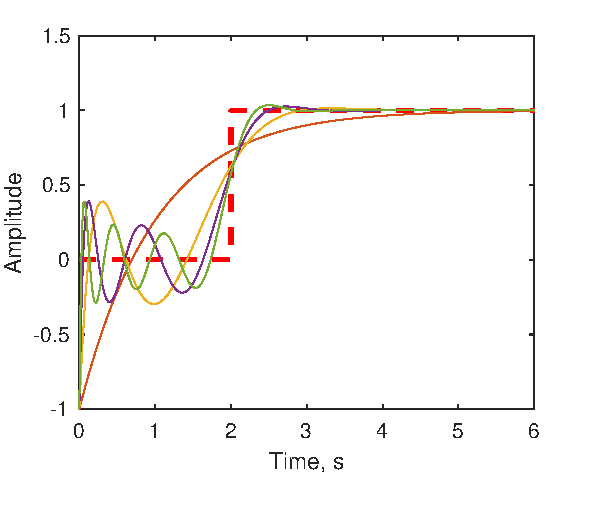
\includegraphics[width=0.5\linewidth]{pade-step.pdf}
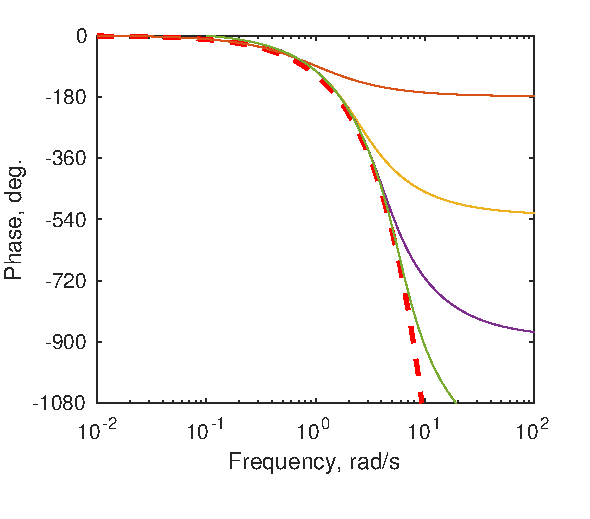
\includegraphics[width=0.5\linewidth]{pade-phase.pdf}}


\end{frame}

\SUBCONCEPT{System Insights from the Bode Plot}

\begin{frame}{Magnitude vs frequency, and phase vs frequency}
  \begin{itemize}
    \item  Used to analyse open loop \emph{and} closed loop
    \item  Frequency is explicit in the graph(s)
    \item  Changes in gain easily interpreted and visualised
    \begin{itemize}
      \item  When inverting just flip
    \end{itemize}
    \item  Time delays and phase lag also easily seen
    \item  Log / dB shows magnitude clearly over many orders of magnitude
\begin{itemize}
  \item Often express $a$ in dB with: $20\log_{10}(a)$
  \item $+\SI{20}{dB} \equiv \times 10$
  \item $-\SI{20}{dB} \equiv \times 0.1$
  \item $+\SI{6}{dB}  \equiv \times 2$
  \item $-\SI{3}{dB}  \equiv \times 1/\sqrt{2} \approx \times 0.707$
\end{itemize}
  \end{itemize}
\end{frame}

\begin{frame}{Resultant properties}
  Use Bode plots to discuss: (non-exhaustive list!)
  \begin{itemize}
    \item  DC gain
    \item  Bandwidth
    \item  Peak response and its frequency
    \item  Low frequency magnitude slope
    \item  High frequency magnitude slope (`roll-off')
    \item  Low frequency phase limit
    \item  High frequency phase limit
  \end{itemize}
\end{frame}


\begin{frame}{The Bode plot gives a quick overview of a system}
Frequency response perspective: the system is a filter which changes the amplitude and phase of an input signal

\vfill
\centering
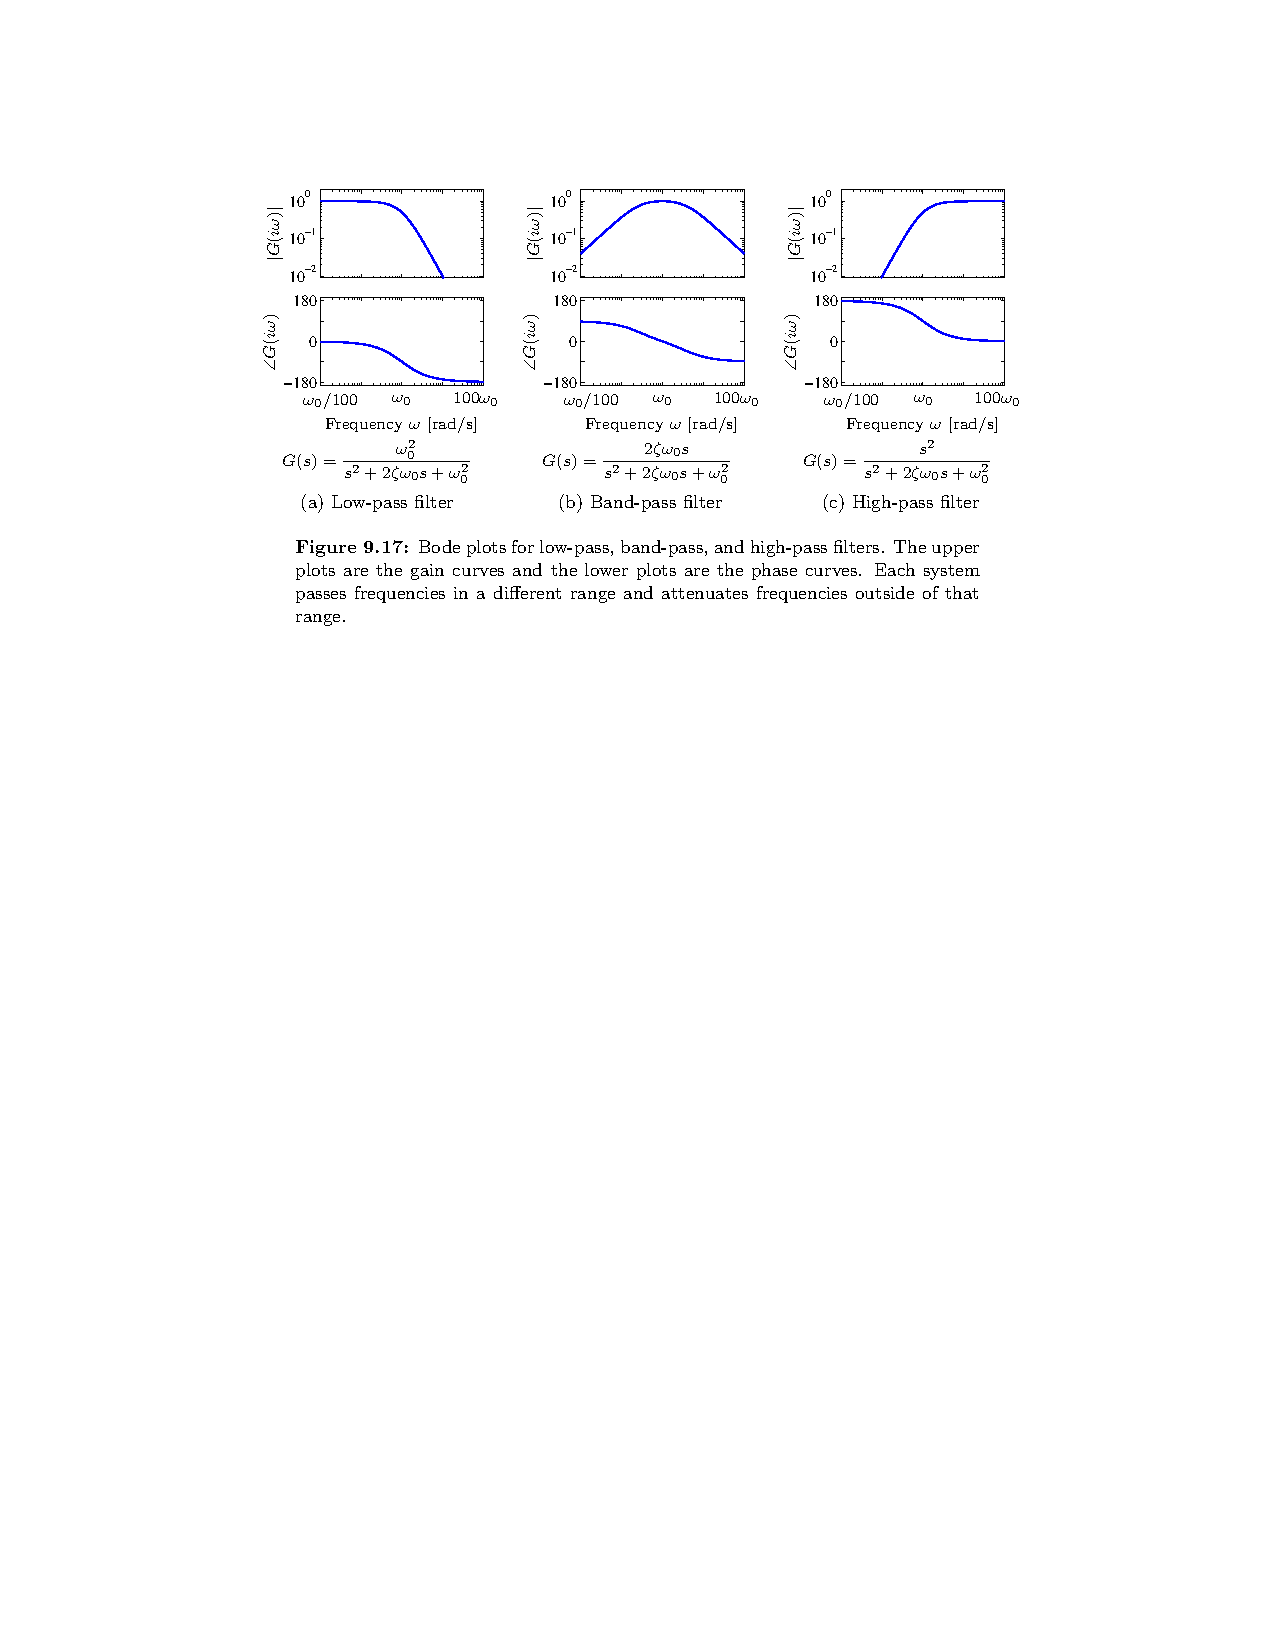
\includegraphics[width=0.8\linewidth]{figure9.17}

\end{frame}

\begin{frame}
\frametitle{Example 9.15 Spring--mass system}

\centering
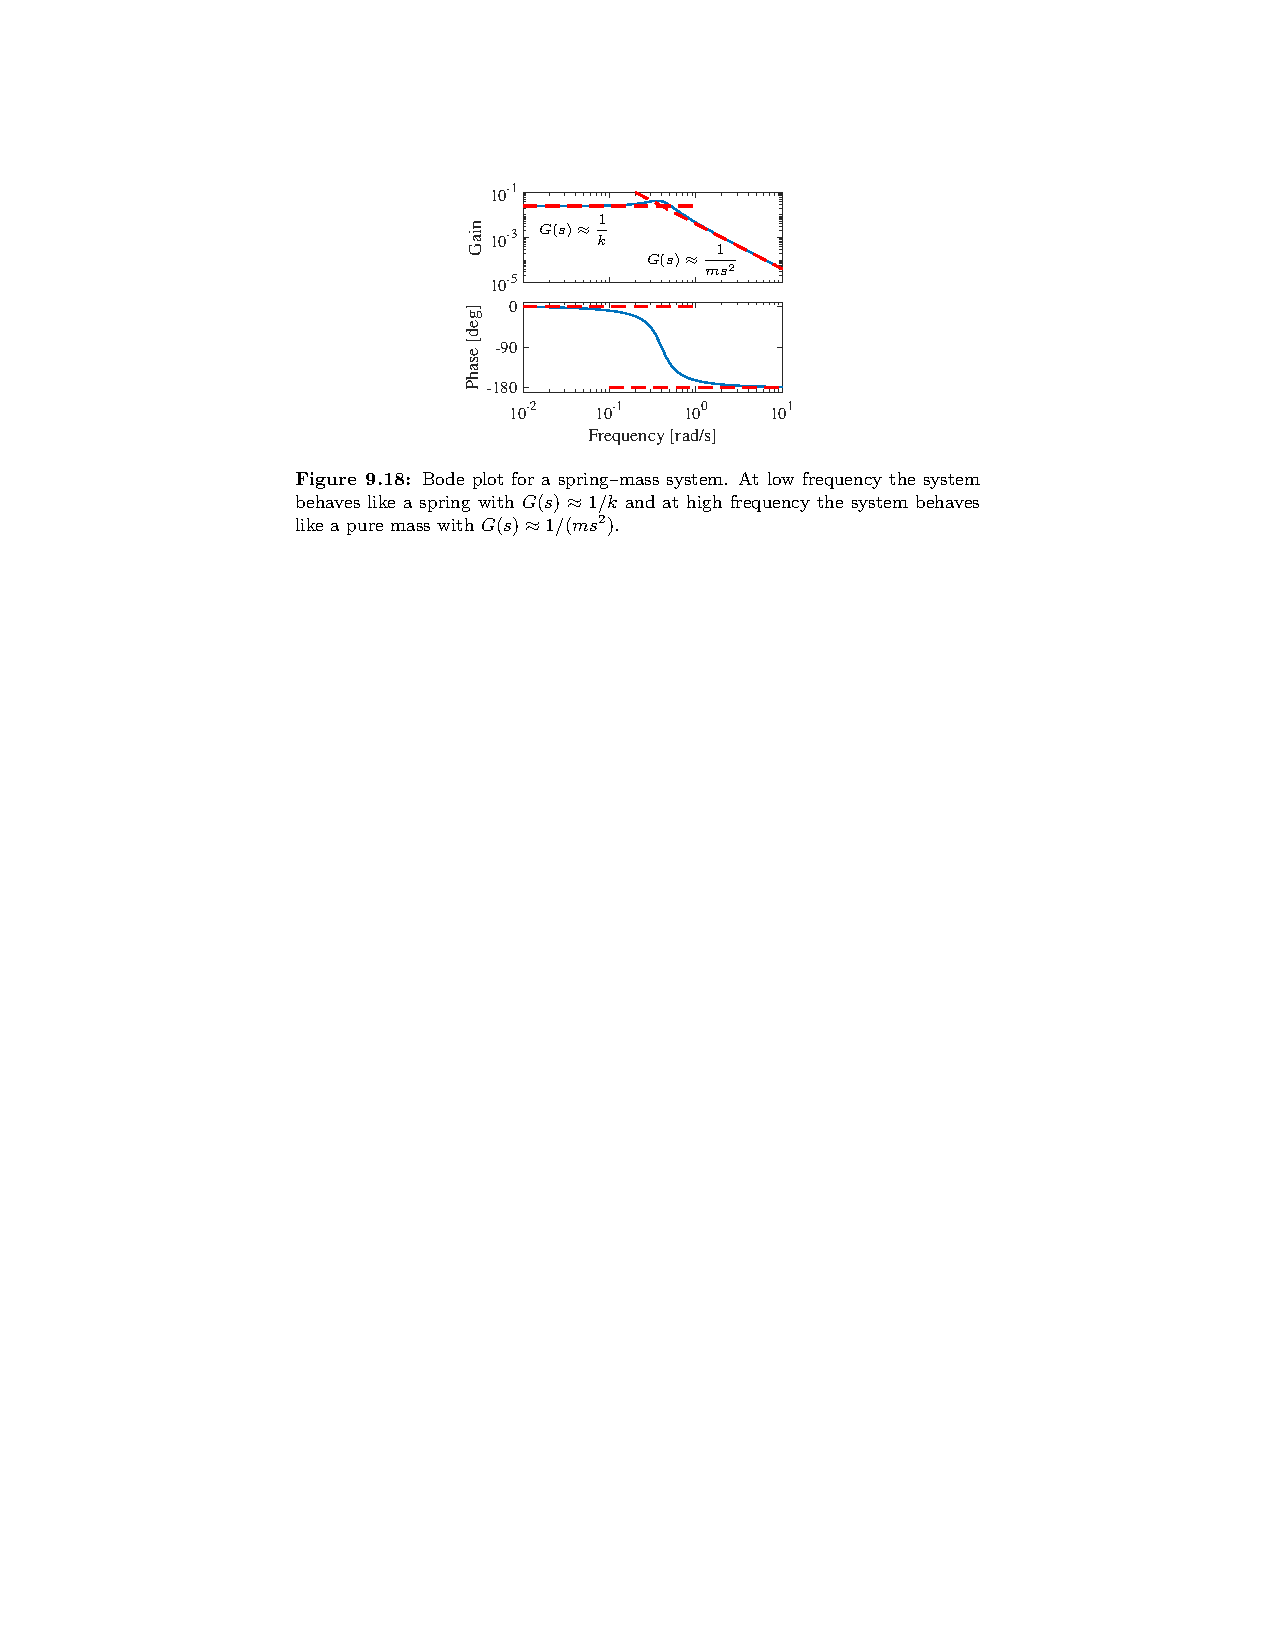
\includegraphics[width=\linewidth]{figure9.18}


\end{frame}


\SUBCONCEPT{Determining Transfer Functions Experimentally}

\begin{frame}{Measuring the FR}
Excite the system in one of three ways:
\begin{itemize}
\item iterate one frequency at a time
\item chirp (ascending or descending or both)
\item white noise
\end{itemize}
The second two methods require the FFT to calculate the FRF:
\begin{itemize}
\item Chirp: FFT size is length of chirp, no windowing
\item Random noise: FFT size as desired, usually use Hanning window
\end{itemize}
Usually avoid using Matlab's \texttt{fft} command --- use \texttt{pwelch} and \texttt{tfestimate} instead.
\end{frame}

\begin{frame}
\frametitle{System identification}
\centering

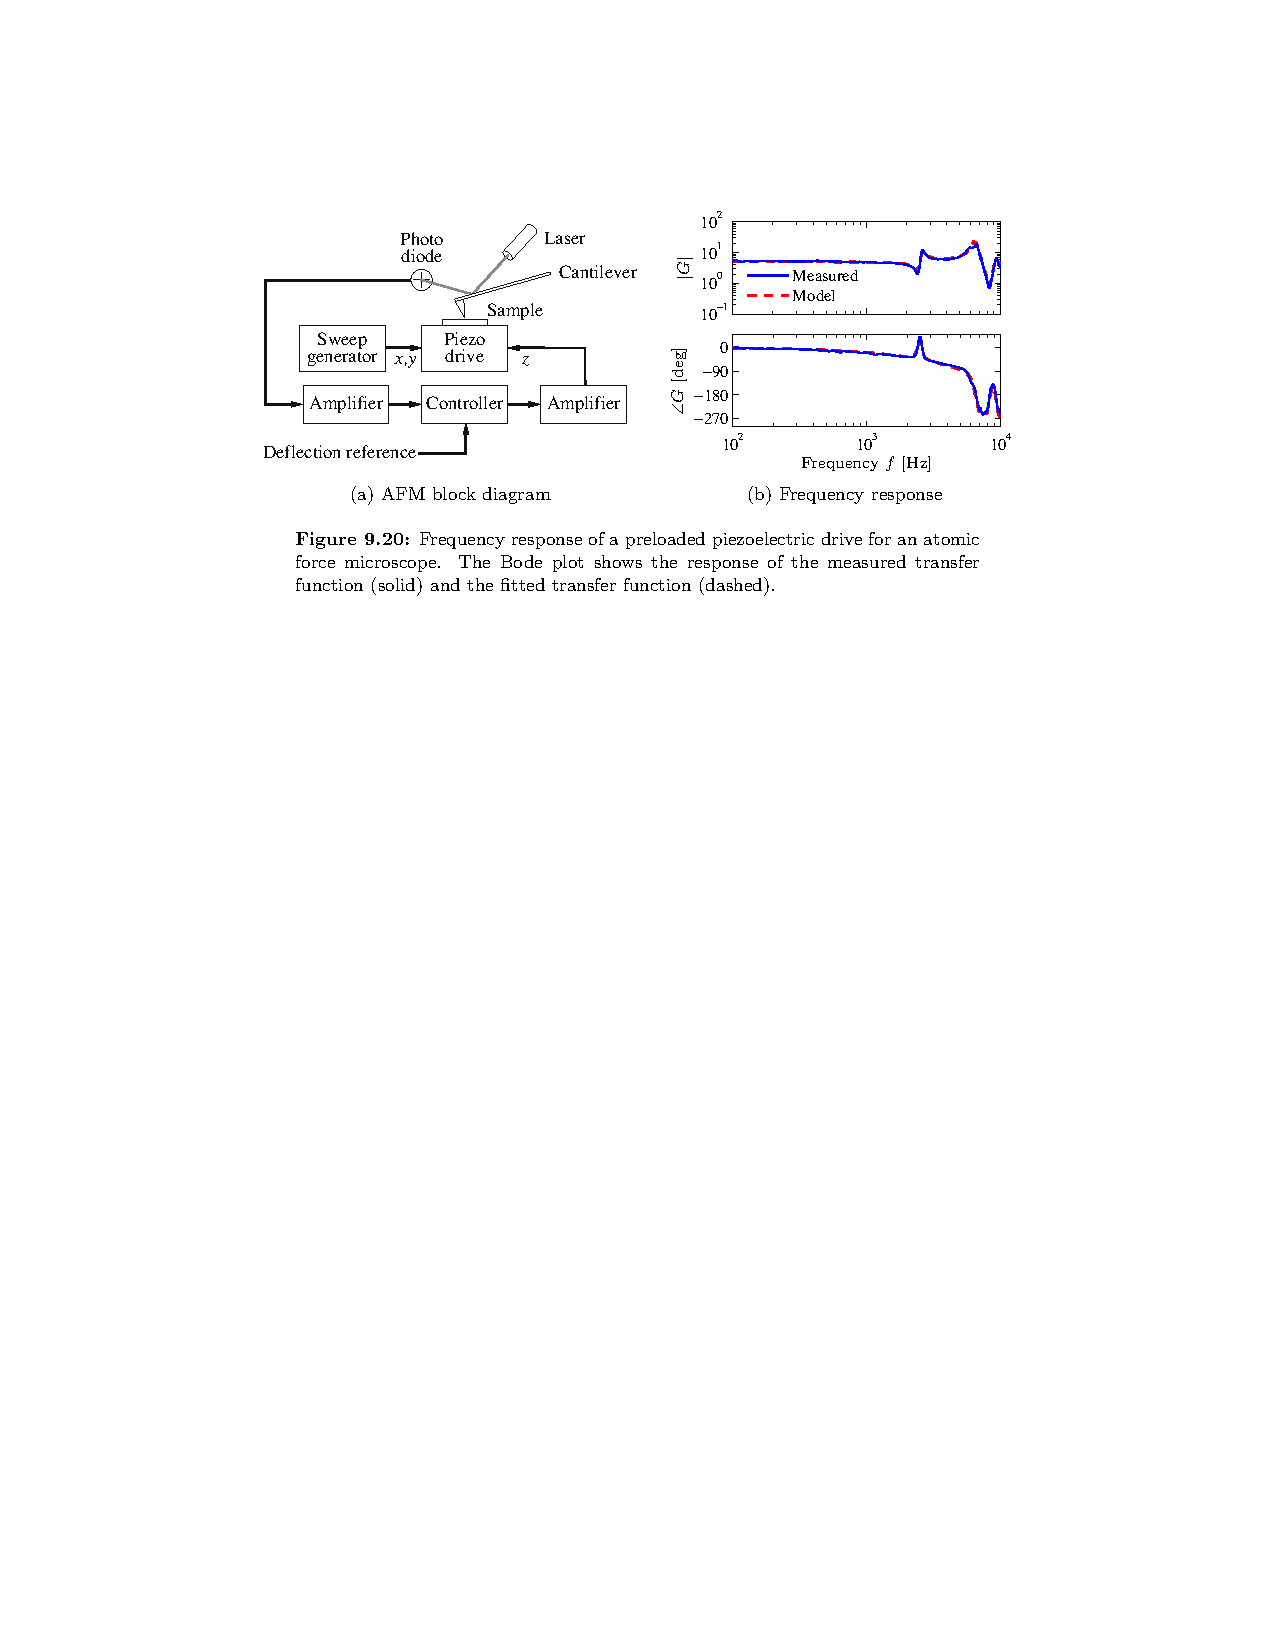
\includegraphics[width=0.7\linewidth]{figure9.20}

\hrulefill
\vfill

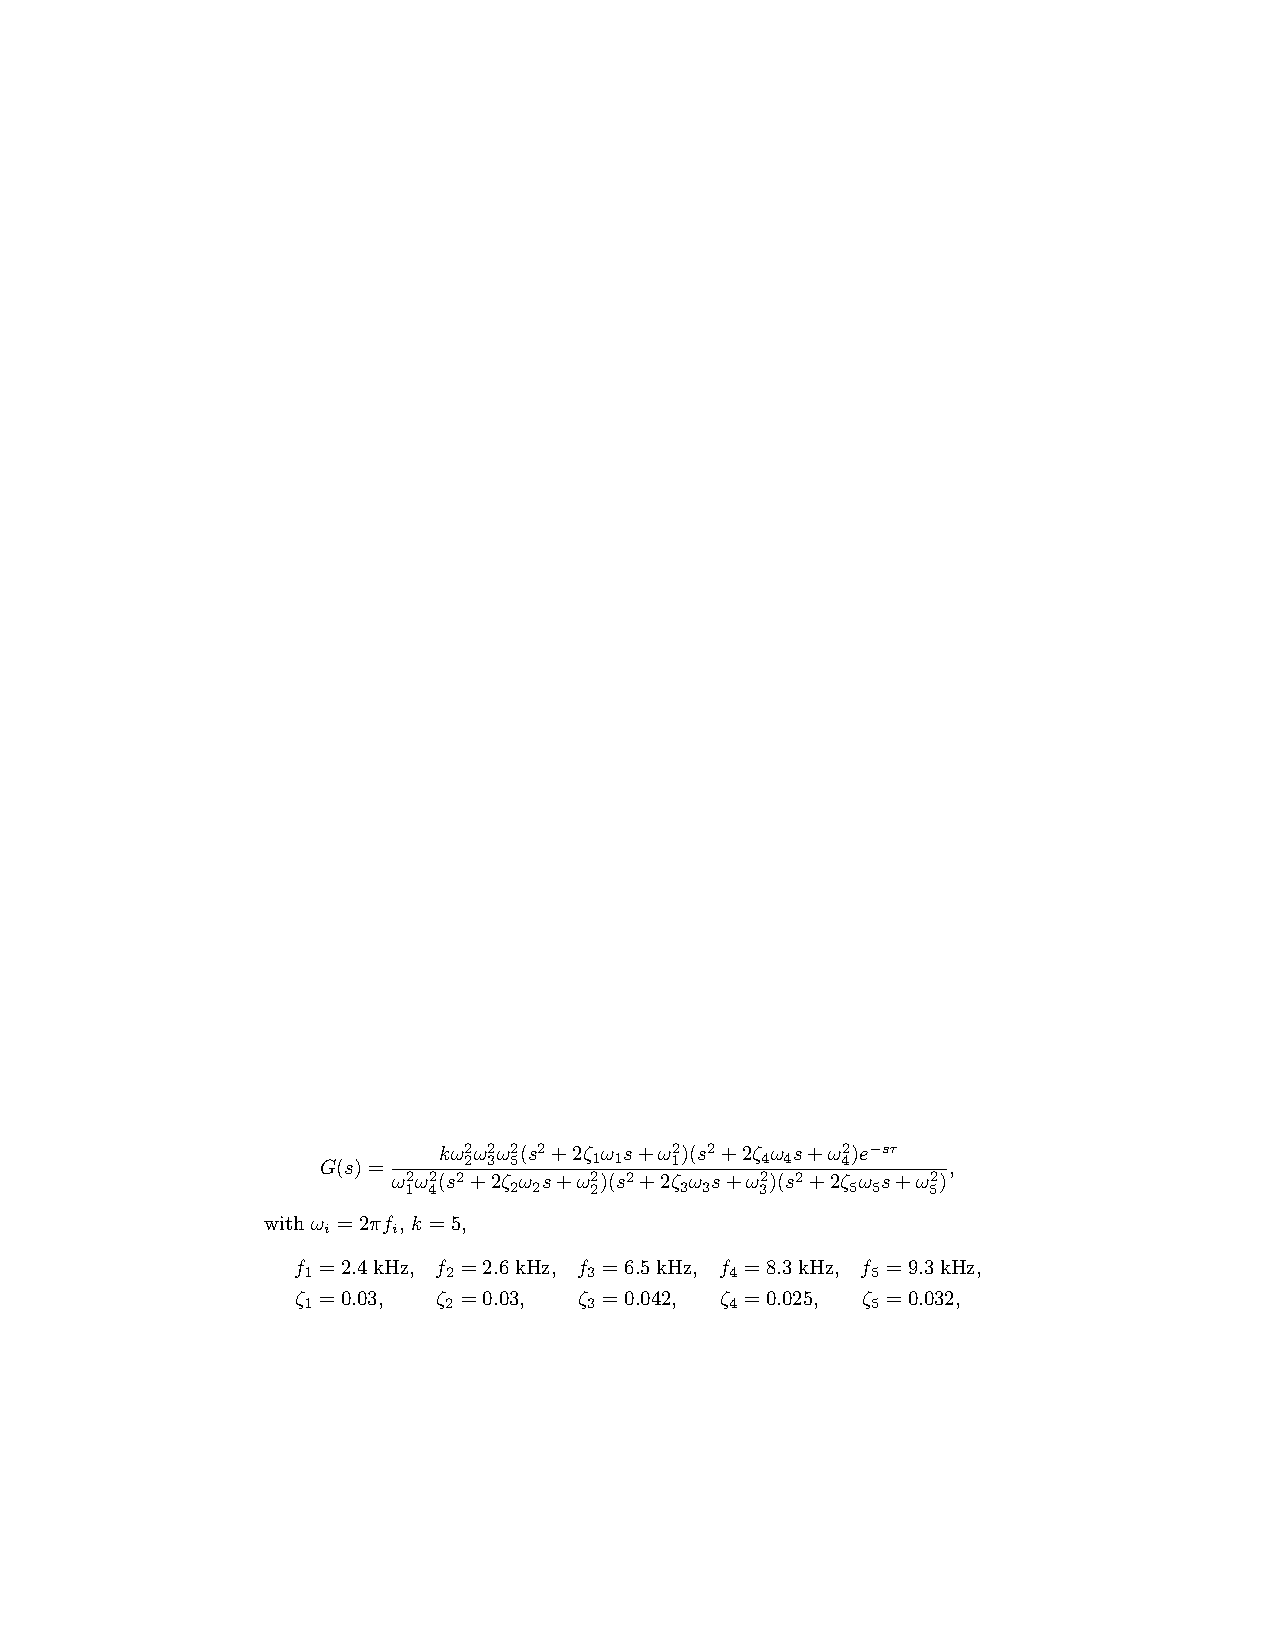
\includegraphics[width=0.7\linewidth]{example9.17}


\end{frame}

\begin{frame}
\frametitle{Matlab example --- sysid from time-domain data}

\begin{columns}
\column{0.5\textwidth}
From System Identification Toolbox: (example in \texttt{doc tfest})
\includematlab{tfest_test.m}{load}

\column{0.5\textwidth}
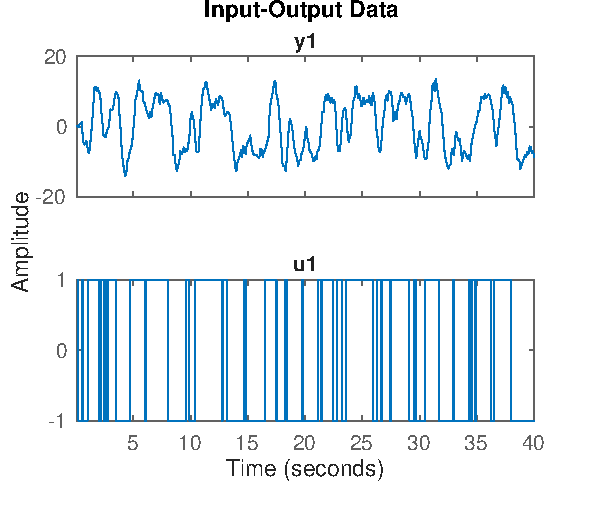
\includegraphics[width=\linewidth]{idtime}

\end{columns}

\end{frame}

\begin{frame}
\frametitle{Matlab example --- sysid from time-domain data}
\small

\begin{columns}
\column{0.5\textwidth}
\includematlab{tfest_test.m}{frf}

\column{0.5\textwidth}
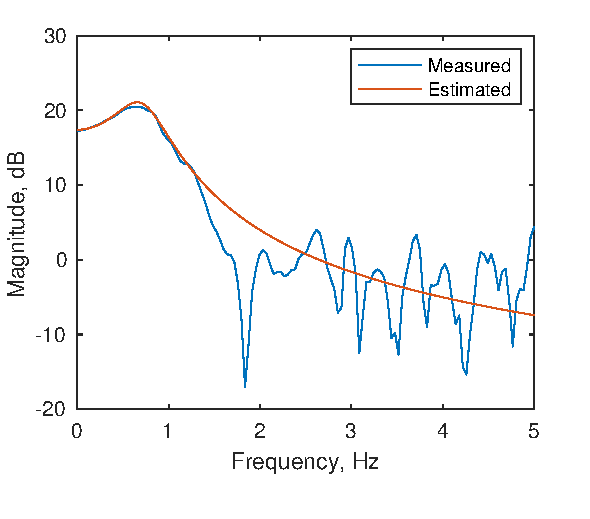
\includegraphics[width=\linewidth]{idfreq}
\end{columns}
\end{frame}

\SUMMARYFRAME
\FINALE

\end{document}



